\begin{frame}{Der VF2 Algorithmus}{}
	\begin{itemize}
	  \item VF2: \\
	    \( (G_1, G_2) \mapsto \begin{cases}
                              \texttt{True},~~ \textit{\small falls \(G_2\) isomorph zu induz. Subgraph von \(G_1\)} \\
                              \texttt{False},~~ \textit{\small sonst}
                            \end{cases}\)
	  \item VF2 ist
	    \begin{itemize}[]
	      \item<.-> allgemein
	      \item<.-> vergleichsweise effizient
	      \item<.-> und erlaubt semantische Matchings
	    \end{itemize}
	    \textit{(Cordella, Foggia, Sansone, Vento)}.
	\end{itemize}
	\begin{figure}
	  \centering
    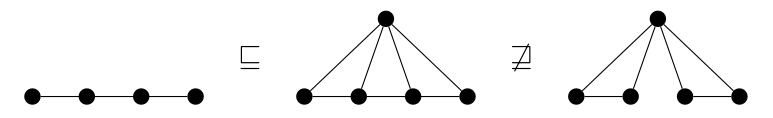
\includegraphics[width=0.7\textwidth]{subisomorphie.png}
	\end{figure}
\end{frame}
